\section{(Introducci\'on) Predicci\'on en el mercado de valores}

Una de las formas más sencillas, y a la vez dif\'iciles, de enriquecerse es la compra de bienes y posterior venta a un precio mayor. La ganacia se produce si se consigue que la diferencia entre el precio de compra y el precio de venta sea mayor que los costes producidos a raz\'on de esa transacci\'on. En el mundo de los negocios la compra y la venta de bienes aparecen en casi todos los sectores econ\'omicos. Por ejemplo:

\begin{itemize}
    \item Distribuci\'on de mercancias. Hay empresas que se dedican a comprar mercancias en un punto y distribuirlas por otras zonas a un precio mayor. El coste de este ejercicio reside en el transporte. La empresa debe asegurar que los costes de transportes no superan a la diferencia de precio entre compra y venta.
    
    \item Especulaci\'on de terrenos o edificios. Un poco m\'as cara que la anterior, la compra, y posterior venta, de edificios puede producir beneficios. Las empresas que se dedican a esto tienen en cuenta las posibles construcciones que se van a hacer por la zona que, posiblemente, elevar\'an el valor del inmueble y har\'an el negocio posible. Mantener terreno conlleva un pago de impuestos, que tendr\'a que ser cubierto con el beneficio de la venta. Pero, en este caso, los inmuebles se pueden alquilar para sacar un beneficio continuo.
\end{itemize}

Del mismo modo, el mercado de valores brinda una posibilidad para extraer beneficio con la compra y venta. Se compran acciones a un precio determinado y se intentan vender a otro m\'as alto. Si se tiene informaci\'on adicional que nos d\'e certeza sobre la subida del precio de la acci\'on entonces el negocio es seguro. Si, por el contrario, no se dispone de informaci\'on, el valor de las acciones podr\'ia bajar y provocar una p\'erdida de dinero.

Por tanto, tener conocimiento sobre el estado del mercado sit\'ua a empresas y particulares en posiciones ventajosas. Es por esto que, siguiendo distintas estrategias, las personas que invierten en bolsa intentan extraer informaci\'on sobre la situaci\'on actual y futura del mercado.\\

A lo largo de este proyecto se va a intentar extraer informaci\'on a partir del hist\'orico de valores del mercado, es decir, vamos a utilizar el estado del mercado en un per\'iodo pasado para predecir el estado futuro. 


\subsection{Precedentes en la predicci\'on de bolsa}
El primer mercado de valores se sit\'ua en el siglo XVII. Seg\'un afirma Beattie (2017) en la revista digital Investopedia, la primera empresa en ofrecer acciones se situar\'ia en B\'elgica, promovida por la incipiente econom\'ia generada en las colonias de Asia. 

A lo largo de tantos a\~nos de vida, los valores burs\'atiles se han intentado predecir de muchas formas. A medida que la sociedad avanza y se van creando nuevas herramientas, los modelos de predicci\'on van evolucionando y se hacen m\'as complejos.

En la actualidad podemos distinguir varias agrupaciones de an\'alisis de bolsa:

\begin{itemize}
    \item \textbf{An\'alisis chartista}. Debe su nombre a la palabra inglesa \textit{chart}. Las estrategias de esta agrupaci\'on se valen de reglas gr\'aficas aplicadas sobre \'indices o sobre el propio valor de la acci\'on. Esas reglas gr\'aficas advierten de series temporales, como las ondas de Elliot (Elliot, 1994), o de tendencias y rupturas (Gartley, 1935). 
    
    Esta estrategia se lleva utilizando mucho tiempo por su simplicidad y su f\'acil comprensi\'on y evaluaci\'on.
    Su \'exito se debe probablemente a este hecho, y es que con una sencilla herramienta gr\'afica se pueden deducir, a gran escala, algunas subidas o bajadas de los valroes de bolsa.
    
    \item \textbf{An\'alisis de \'indices o indicadores}. Esta modalidad de an\'alisis se basa en el uso de estad\'isticos. En el campo de la estad\'istica, los estad\'isticos son valores que representan una determinada caracter\'istica de la variable a la que refiere. En el caso de los indicadores, informan del estado de uno o varios valores distintos de la bolsa. Una de las publicaciones con m\'as renombre es la teor\'ia de Dow\footnote{Hamilton, W. P. (1922). \textit{The Stock Market Barometer; a Study of Its Forecast Value Based on Charles H. Dow's Theory of the Price Movement}, Harper \& Bros., Nueva York}, cuyo autor, Charles H. Dow, fue el fundador del \textit{Wall Street Journal}, diario en el que publicaba sus principios para invertir en bolsa. 
    
    Seg\'un la variable que resume el indicador podemos hablar de varios tipos. El primer tipo son los indicadores que representan la situaci\'on general de la bolsa de un pa\'is, por ejemplo el IBEX35 (35 empresas con m\'as capital de Espa\~na). Otro grupo de indicadores son los representan la situaci\'on de las empresas que se dedican a un sector particular, como el  SX7E (bancos de los paises europeos).
    Por \'ultimo hay \'indicadores que aportan informaci\'on estad\'istica sobre un solo valor, por ejemplo la EMA (Media M\'ovil Exponencial).
\end{itemize}

Este proyecto se centra en el an\'alisis de indicadores de un solo valor. En concreto, como se ver\'a a lo largo del trabajo, se propone un modelo basado en \'arboles de decisi\'on construidos a partir de un algoritmo gen\'etico. Los \'arboles de decisi\'on son, a grandes rasgos, estructuras que permiten crear una jerarqu\'ia de condiciones que tienen como conclusi\'on de las mismas una clasificaci\'on. En el caso que nos compete, la clasificaci\'on corresponder\'a a decidir si es un buen momento para comprar, para vender o para ninguno de los dos. En el apartado \ref{sec:algorithm} se entrar\'a con m\'as profundidad en este modelo. 



\subsection{Tipos de informaci\'on extra\'ible a partir de \'arboles}
Podemos encontrar en la bibliograf\'ia varios modelos basados en \'arboles que, seg\'un la informaci\'on que persiguen conseguir, se pueden dividir en varios grupos. En este punto debemos hacer notar que existen otras formas y herramientas de extracci\'on informaci\'on o predecci\'on, pero por la naturaleza de nuestra propuesta nos centraremos en las estrategias basadas en \'arboles. Debido al caracter motivacional de la secci\'on, no se entra en profundidad en estos conceptos. No obstante, la definici\'on de \'arbol puede verse posteriormente en el apartado \ref{sec:Decision_tree}.

    \subsubsection{Informaci\'on total}
    
    El m\'as ambicioso de los objetivos de un an\'alisis de bolsa es el de encontrar una forma de predecir el valor exacto de un valor burs\'atil en un instante de tiempo futuro. Encontramos entonces una funci\'on $f:\Omega \rightarrow \mathbb{R}$ donde $\Omega$ es un conjunto de indicadores del valor a predecir en un instante pasado o presente y la imagen, contenida en $\mathbb{R}$ es el valor predicho para un instante en el futuro.
    
    El instante predicho cambia seg\'un el autor del estudio (pueden ser horas, d\'ias o semanas), normalmente, cuanto m\'as alejado est\'a del instante en el que se eval\'ua $f$ del instante que se pretende predecir, mayor es el error.\\
    
    La funci\'on $f$ se puede representar como un \'arbol en el que en los nodos se sit\'uan operaciones (usualmente unarias o binarias) y las hojas contienen par\'ametros de la funci\'on $f$ o valores constantes. La funci\'on se eval\'ua desde las hojas hasta el nodo ra\'iz. \\
    
	\begin{figure}[H]
		\centering
    	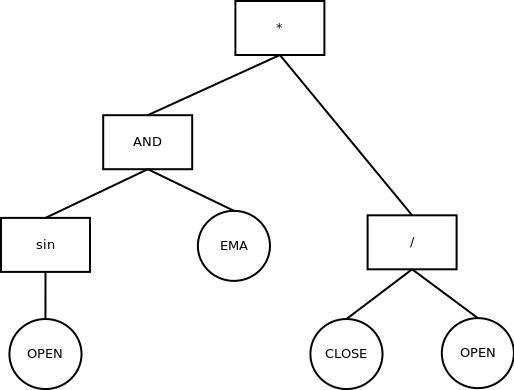
\includegraphics[scale=0.5]{imagenes/arbol_inf_comp.png}
    	\caption[Ejemplo de \'arbol de programaci\'on gen\'etica]{Ejemplo de \'arbol de programaci\'on gen\'etica.\\ Fuente: elaboraci\'on propia.}
    	\label{fig:inf_compl}
    \end{figure}
    
    En la figura \ref{fig:inf_compl} puede verse un \'arbol de este tipo. De este se puede extraer la funci\'on \\
    $f($OPEN, CLOSE, EMA$) = (sin($OPEN$)$ AND EMA$) * ($CLOSE/OPEN$)$\\ que, dados unos valores para la apertura, el cierre y la media m\'ovil exponencial, nos devuelve el valor en el instante futuro.\\
    
    Para ajustar los \'arboles se usa un algoritmo gen\'etico con funci\'on \textit{fitness} el error medio cuadr\'atico entre el valor predicho y el error real (Sheta, 2013). Se comentar\'a con profundidad el funcionamiento de los algoritmos gen\'eticos m\'as adelante. Tambi\'en existe otra variante basada en el \textit{Conditional Sharpe Ratio} aplicada en Esfahanipour (2011) y Mousavi (2014).
    
    Por \'ultimo, una funci\'on \textit{fitness} algo diferente es puntuar cada estrategia a partir del beneficio simulado obtenido en un periodo de tiempo (Potvin, 2004).
    
     Si se consiguiese hallar una funci\'on $f$ con un error nulo, obtendriamos una informaci\'on perfecta con la que podr\'iamos conseguir el m\'aximo beneficio en bolsa. No obstante, este tipo de modelos es demasiado ambicioso. Computacionalmente es pesado y la funci\'on resultante no es, en casi todos los casos, interpretable.
     
     
     \subsubsection{Informaci\'on de tendencias}
     
     En lugar de buscar una predicci\'on exacta del valor en el futuro, podemos estar interesados en obtener informaci\'on sobre la tendencia de un valor, es decir, si est\'a en un periodo ascendente o descendente. \\
     
     Este m\'etodo puede ser visto como una relajaci\'on del m\'etodo desarrollado en el apartado anterior. Aunque el paso de una imagen continua ($\mathbb{R}$) a una imagen discreta (sube, baja, se queda igual) nos obliga a realizar otro tipo de \'arboles. En este caso se suele proponer un \'arbol de decisi\'on con tres etiquetas. Pero no vamos a entrar en detalle aqu\'i en esta herramienta, ya que ser\'a explicada en profundidad en el apartado \ref{sec:Decision_tree}.\\
     
     Estos modelos de informaci\'on son bastante m\'as sencillos de interpretar. Pero, por contra, son bastante m\'as imprecisos. El modelo nos dice la tendencia que tendr\'a el valor. Sin embargo, seg\'un los objetivos de inversi\'on, las comisiones u otras situaciones econ\'omicas, esta informaci\'on podr\'ia no ser suficiente para sacar beneficios.\\
     
     Para profundizar en la extracci\'on de este tipo de informaci\'on se sugiere ver Nair (2010) o Huang (2008).
     
     
     \subsubsection{Informaci\'on de se\~nales de compra y venta}
     
     A medio camino entre los dos tipos de informaci\'on anteriores tenemos los modelos de señales, mediante los cuales, los m\'as importante no es conocer el valor de la acci\'on, si sube o si baja, sino buscar un modelo que nos diga cuando comprar y cuando vender. A estas advertencias de los modelos de compra y venta se le llaman se\~nales de compra y venta. Cabe decir que se puede hacer una extensi\'on del modelo para que no tenga una decisi\'on binaria, por ejemplo un modelo de cuatro etiquetas: compra discreta, venta discreta, compra masiva y venta masiva. \\
     
     De este tipo de extracci\'on de informaci\'on hay menos ejemplos, que suelen estar ejecutados a partir de varios \'arboles de salida booleana, cada uno de ellos asociado a una se\~nal. En Myszkowski (2010) podemos ver un claro ejemplo con dos \'arboles, uno que indica la compra y otro que indica la venta.
     
     	\begin{figure}[H]
			\centering\leftskip=-10px
			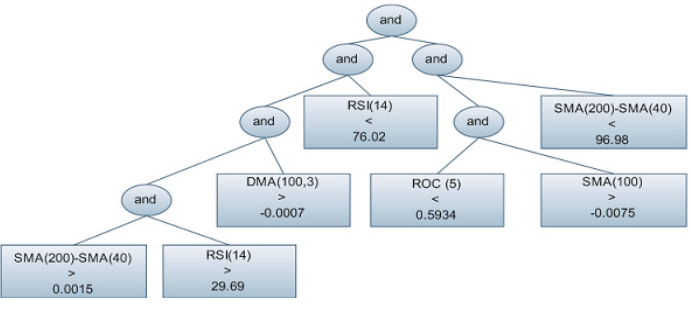
\includegraphics[scale=0.8]{imagenes/tree_halfinfo.png}
			\caption[Ejemplo de \'arbol de señales de compra]{Ejemplo de \'arbol de señales de compra. \\Fuente: Myszkowski (2010)}
			\label{fig:tree_half_info}
		\end{figure}
		
	En la figura \ref{fig:tree_half_info} se muestra un \'arbol de se\~nal de compra. N\'otese que en los nodos hoja siempre hay una condici\'on booleana que puede contener un solo indicador o, en caso especial, dos.
	
	\subsection{Objetivo del proyecto}
	La importancia de obtener informaci\'on exclusiva sobre el estado de la bolsa es evidente, ya que esto te permite invertir en bolsa con mayor posibilidad de sacar beneficios que si se realizara por mera intuici\'on.\\
	
	De este modo, siguiendo el desarrollo realizado en los antecedentes aportados, se propone conseguir los siguientes objetivos principales:
	
	\begin{itemize}
	    \item Dise\~nar un algoritmo gen\'etico basado en \'arboles que permita extraer informaci\'on de se\~nales de compra y venta.
	    \item Debido al coste computacional de los algoritmos gen\'eticos, se busca implementar dicho algoritmo de la forma m\'as eficiente posible, en especial la funci\'on de evaluaci\'on.
	    \item Ejecutar en distintas tendencias burs\'atiles y comparar los resultados con los aportados en la bibliograf\'ia.
	\end{itemize}
	
	A pesar de que el hist\'orico de datos es clave para predecir los valores futuros, el mercado de valores a menudo se ve influenciado por otros factores no predecibles (noticias, pol\'itica, guerras o cat\'astrofes ambientales, por ejemplo). Por tanto, aunque el modelo predicho sea muy bueno, siempre habr\'a un punto de incertidumbre que nunca estaremos en condiciones de analizar.
	
	En consecuencia, partimos de la idea de que la inversi\'on perfecta no se puede conseguir, al menos de forma juiciosa y sistem\'atica. No obstante, a\~nadimos un punto adicional a los objetivos que, a priori, es complicado alcanzar:
	
	\begin{itemize}
	    \item Mejorar los resultados obtenidos en los distintos mercados de valores de la bibliograf\'ia.
	\end{itemize}
	
	